%% pscc2022_template.tex, V1.1, 2019/03/11
%% by Mario Paolone
%% This is a Latex template to prepare submissions for the PSCC 2022 conference. 
%% The template demonstrates the use of the class IEEEtran4PSCC.cls and is mostly
%% based on the file bare_conf.tex (V1.4a) by Michael Shell.

%%*************************************************************************
%% Legal Notice:
%% This code is offered as-is without any warranty either expressed or
%% implied; without even the implied warranty of MERCHANTABILITY or
%% FITNESS FOR A PARTICULAR PURPOSE! 
%% User assumes all risk.
%% In no event shall PSCC or any contributor to this code be liable for
%% any damages or losses, including, but not limited to, incidental,
%% consequential, or any other damages, resulting from the use or misuse
%% of any information contained here.
%%
%% All comments are the opinions of their respective authors and are not
%% necessarily endorsed by the PSCC.
%%
%% This work is distributed under the LaTeX Project Public License (LPPL)
%% ( http://www.Latex-project.org/ ) version 1.3, and may be freely used,
%% distributed and modified. A copy of the LPPL, version 1.3, is included
%% in the base LaTeX documentation of all distributions of LaTeX released
%% 2003/12/01 or later.
%% Retain all contribution notices and credits.
%% ** Modified files should be clearly indicated as such, including  **
%% ** renaming them and changing author support contact information. **
%%
%% File list of work: pscc2022_template.tex, IEEEtran4PSCC.cls
%%*************************************************************************


% *** Authors should verify (and, if needed, correct) their LaTeX system  ***
% *** with the testflow diagnostic prior to trusting their LaTeX platform ***
% *** with production work.                 ***


\documentclass{IEEEtran4PSCC}
% The automatically selected options are the format (US letter) and conference mode.


% Some very useful LaTeX packages include:
% (uncomment the ones you want to load)
% *** MISC UTILITY PACKAGES ***
%
%\usepackage{ifpdf}
% Heiko Oberdiek's ifpdf.sty is very useful if you need conditional
% compilation based on whether the output is pdf or dvi.
% usage:
% \ifpdf
%   % pdf code
% \else
%   % dvi code
% \fi
% The latest version of ifpdf.sty can be obtained from:
% http://www.ctan.org/tex-archive/macros/Latex/contrib/oberdiek/
% Also, note that IEEEtran.cls V1.7 and later provides a builtin
% \ifCLASSINFOpdf conditional that works the same way.
% When switching from Latex to pdfLatex and vice-versa, the compiler may
% have to be run twice to clear warning/error messages.

% *** CITATION PACKAGES ***
%
%\usepackage{cite}
% cite.sty was written by Donald Arseneau
% V1.6 and later of IEEEtran pre-defines the format of the cite.sty package
% \cite{} output to follow that of IEEE. Loading the cite package will
% result in citation numbers being automatically sorted and properly
% 'compressed/ranged'. e.g., [1], [9], [2], [7], [5], [6] without using
% cite.sty will become [1], [2], [5]--[7], [9] using cite.sty. cite.sty's
% \cite will automatically add leading space, if needed. Use cite.sty's
% noadjust option (cite.sty V3.8 and later) if you want to turn this off
% such as if a citation ever needs to be enclosed in parenthesis.
% cite.sty is already installed on most LaTeX systems. Be sure and use
% version 5.0 (2009-03-20) and later if using hyperref.sty.
% The latest version can be obtained at:
% http://www.ctan.org/tex-archive/macros/Latex/contrib/cite/
% The documentation is contained in the cite.sty file itself.


% *** GRAPHICS RELATED PACKAGES ***
%
\ifCLASSINFOpdf
   \usepackage[pdftex]{graphicx}
  % declare the path(s) where your graphic files are
  % \graphicspath{{../pdf/}{../jpeg/}}
  % and their extensions so you won't have to specify these with
  % every instance of \includegraphics
  % \DeclareGraphicsExtensions{.pdf,.jpeg,.png}
\else
  % or other class option (dvipsone, dvipdf, if not using dvips). graphicx
  % will default to the driver specified in the system graphics.cfg if no
  % driver is specified.
   \usepackage[dvips]{graphicx}
  % declare the path(s) where your graphic files are
  % \graphicspath{{../eps/}}
  % and their extensions so you won't have to specify these with
  % every instance of \includegraphics
  % \DeclareGraphicsExtensions{.eps}
\fi
% graphicx was written by David Carlisle and Sebastian Rahtz. It is
% required if you want graphics, photos, etc. graphicx.sty is already
% installed on most LaTeX systems. The latest version and documentation
% can be obtained at: 
% http://www.ctan.org/tex-archive/macros/Latex/required/graphics/
% Another good source of documentation is 'Using Imported Graphics in
% LaTeX2e' by Keith Reckdahl which can be found at:
% http://www.ctan.org/tex-archive/info/epsLatex/
%
% Latex, and pdfLatex in dvi mode, support graphics in encapsulated
% postscript (.eps) format. pdfLatex in pdf mode supports graphics
% in .pdf, .jpeg, .png and .mps (metapost) formats. Users should ensure
% that all non-photo figures use a vector format (.eps, .pdf, .mps) and
% not a bitmapped formats (.jpeg, .png). IEEE frowns on bitmapped formats
% which can result in 'jaggedy'/blurry rendering of lines and letters as
% well as large increases in file sizes.
%
% You can find documentation about the pdfTeX application at:
% http://www.tug.org/applications/pdftex



% *** MATH PACKAGES ***
%
\usepackage[cmex10]{amsmath}
% A popular package from the American Mathematical Society that provides
% many useful and powerful commands for dealing with mathematics. If using
% it, be sure to load this package with the cmex10 option to ensure that
% only type 1 fonts will utilized at all point sizes. Without this option,
% it is possible that some math symbols, particularly those within
% footnotes, will be rendered in bitmap form which will result in a
% document that can not be IEEE Xplore compliant!
%
% Also, note that the amsmath package sets \interdisplaylinepenalty to 10000
% thus preventing page breaks from occurring within multiline equations. Use:
%\interdisplaylinepenalty=2500
% after loading amsmath to restore such page breaks as IEEEtran.cls normally
% does. amsmath.sty is already installed on most LaTeX systems. The latest
% version and documentation can be obtained at:
% http://www.ctan.org/tex-archive/macros/Latex/required/amsLatex/math/





% *** SPECIALIZED LIST PACKAGES ***
%
% \usepackage{algorithmic}
% algorithmic.sty was written by Peter Williams and Rogerio Brito.
% This package provides an algorithmic environment fo describing algorithms.
% You can use the algorithmic environment in-text or within a figure
% environment to provide for a floating algorithm. Do NOT use the algorithm
% floating environment provided by algorithm.sty (by the same authors) or
% algorithm2e.sty (by Christophe Fiorio) as IEEE does not use dedicated
% algorithm float types and packages that provide these will not provide
% correct IEEE style captions. The latest version and documentation of
% algorithmic.sty can be obtained at:
% http://www.ctan.org/tex-archive/macros/Latex/contrib/algorithms/
% There is also a support site at:
% http://algorithms.berlios.de/index.html
% Also of interest may be the (relatively newer and more customizable)
% algorithmicx.sty package by Szasz Janos:
% http://www.ctan.org/tex-archive/macros/Latex/contrib/algorithmicx/




% *** ALIGNMENT PACKAGES ***
%
%\usepackage{array}
% Frank Mittelbach's and David Carlisle's array.sty patches and improves
% the standard LaTeX2e array and tabular environments to provide better
% appearance and additional user controls. As the default LaTeX2e table
% generation code is lacking to the point of almost being broken with
% respect to the quality of the end results, all users are strongly
% advised to use an enhanced (at the very least that provided by array.sty)
% set of table tools. array.sty is already installed on most systems. The
% latest version and documentation can be obtained at:
% http://www.ctan.org/tex-archive/macros/Latex/required/tools/


% IEEEtran contains the IEEEeqnarray family of commands that can be used to
% generate multiline equations as well as matrices, tables, etc., of high
% quality.




% *** SUBFIGURE PACKAGES ***
%\ifCLASSOPTIONcompsoc
%  \usepackage[caption=false,font=normalsize,labelfont=sf,textfont=sf]{subfig}
%\else
%  \usepackage[caption=false,font=footnotesize]{subfig}
%\fi
% subfig.sty, written by Steven Douglas Cochran, is the modern replacement
% for subfigure.sty, the latter of which is no longer maintained and is
% incompatible with some LaTeX packages including fixltx2e. However,
% subfig.sty requires and automatically loads Axel Sommerfeldt's caption.sty
% which will override IEEEtran.cls' handling of captions and this will result
% in non-IEEE style figure/table captions. To prevent this problem, be sure
% and invoke subfig.sty's 'caption=false' package option (available since
% subfig.sty version 1.3, 2005/06/28) as this is will preserve IEEEtran.cls
% handling of captions.
% Note that the Computer Society format requires a larger sans serif font
% than the serif footnote size font used in traditional IEEE formatting
% and thus the need to invoke different subfig.sty package options depending
% on whether compsoc mode has been enabled.
%
% The latest version and documentation of subfig.sty can be obtained at:
% http://www.ctan.org/tex-archive/macros/Latex/contrib/subfig/




% *** FLOAT PACKAGES ***
%
%\usepackage{fixltx2e}
% fixltx2e, the successor to the earlier fix2col.sty, was written by
% Frank Mittelbach and David Carlisle. This package corrects a few problems
% in the LaTeX2e kernel, the most notable of which is that in current
% LaTeX2e releases, the ordering of single and double column floats is not
% guaranteed to be preserved. Thus, an unpatched LaTeX2e can allow a
% single column figure to be placed prior to an earlier double column
% figure. The latest version and documentation can be found at:
% http://www.ctan.org/tex-archive/macros/Latex/base/


%\usepackage{stfloats}
% stfloats.sty was written by Sigitas Tolusis. This package gives LaTeX2e
% the ability to do double column floats at the bottom of the page as well
% as the top. (e.g., '\begin{figure*}[!b]' is not normally possible in
% LaTeX2e). It also provides a command:
%\fnbelowfloat
% to enable the placement of footnotes below bottom floats (the standard
% LaTeX2e kernel puts them above bottom floats). This is an invasive package
% which rewrites many portions of the LaTeX2e float routines. It may not work
% with other packages that modify the LaTeX2e float routines. The latest
% version and documentation can be obtained at:
% http://www.ctan.org/tex-archive/macros/Latex/contrib/sttools/
% Do not use the stfloats baselinefloat ability as IEEE does not allow
% \baselineskip to stretch. Authors submitting work to the IEEE should note
% that IEEE rarely uses double column equations and that authors should try
% to avoid such use. Do not be tempted to use the cuted.sty or midfloat.sty
% packages (also by Sigitas Tolusis) as IEEE does not format its papers in
% such ways.
% Do not attempt to use stfloats with fixltx2e as they are incompatible.
% Instead, use Morten Hogholm'a dblfloatfix which combines the features
% of both fixltx2e and stfloats:
%
% \usepackage{dblfloatfix}
% The latest version can be found at:
% http://www.ctan.org/tex-archive/macros/Latex/contrib/dblfloatfix/




% *** PDF, URL AND HYPERLINK PACKAGES ***
%
% \usepackage{url}
% url.sty was written by Donald Arseneau. It provides better support for
% handling and breaking URLs. url.sty is already installed on most LaTeX
% systems. The latest version and documentation can be obtained at:
% http://www.ctan.org/tex-archive/macros/Latex/contrib/url/
% Basically, \url{my_url_here}.




% *** Do not adjust lengths that control margins, column widths, etc. ***
% *** Do not use packages that alter fonts (such as psLatex).         ***
% There should be no need to do such things with IEEEtran.cls V1.6 and later.


% correct bad hyphenation here
\hyphenation{op-tical net-works semi-conduc-tor}



% Set footer
\makeatletter
\let\old@ps@headings\ps@headings
\let\old@ps@IEEEtitlepagestyle\ps@IEEEtitlepagestyle
\def\psccfooter#1{%
    \def\ps@headings{%
        \old@ps@headings%
        \def\@oddfoot{\strut\hfill#1\hfill\strut}%
        \def\@evenfoot{\strut\hfill#1\hfill\strut}%
    }%
    \def\ps@IEEEtitlepagestyle{%
        \old@ps@IEEEtitlepagestyle%
        \def\@oddfoot{\strut\hfill#1\hfill\strut}%
        \def\@evenfoot{\strut\hfill#1\hfill\strut}%
    }%
    \ps@headings%
}
\makeatother

\psccfooter{%
        \parbox{\textwidth}{\hrulefill \\ \small{22nd Power Systems Computation Conference} \hfill \begin{minipage}{0.2\textwidth}\centering \vspace*{4pt} 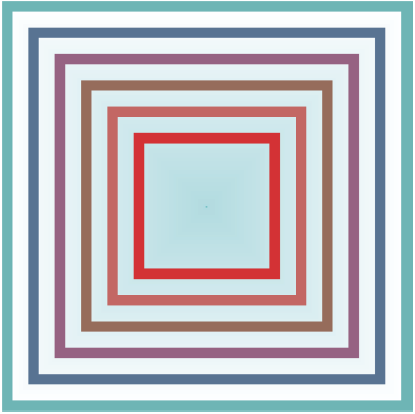
\includegraphics[scale=0.06]{PSCC_logo.png}\\\small{PSCC 2022} \end{minipage} \hfill \small{Porto, Portugal --- June 27 -- July 1, 2022}}%
}

\usepackage{lipsum}
\begin{document}

\newcommand{\packageName}{PowerEdu.jl}

%
% paper title
% Titles are generally capitalized except for words such as a, an, and, as,
% at, but, by, for, in, nor, of, on, or, the, to and up, which are usually
% not capitalized unless they are the first or last word of the title.
% Linebreaks \\ can be used within to get better formatting as desired.
% Do not put math or special symbols in the title.
\title{\packageName{} - A Julia Package for Teaching Power System Courses}



%% To specify the authors when (number of affiliations <= 2)
\author{
\IEEEauthorblockN{Ninad Gaikwad, Aryan Jha, Sajjad Uddin Mahmud, Anamika Dubey, Noel Schulz, and Mani Venkatasubramanian}
\IEEEauthorblockA{School of Electrical Engineering \& Computer Science, Washington State University, Pullman, WA, USA\\
\{ninad.gaikwad, aryan.jha, sajjaduddin.mahmud, anamika.dubey, noel.schulz, mani\}@wsu.edu}}

%% To specify the authors when (number of affiliations > 2)
% \author{\IEEEauthorblockN{Author n.1\IEEEauthorrefmark{1},
% Author n.2\IEEEauthorrefmark{2},
% Author n.3\IEEEauthorrefmark{3}, 
% Author n.4\IEEEauthorrefmark{3} and
% Author n.5\IEEEauthorrefmark{4}}
% \IEEEauthorblockA{\IEEEauthorrefmark{1} Department Name of Organization A\\
% Name of the organization A,
% Address A\\ Emails if wanted}
% \IEEEauthorblockA{\IEEEauthorrefmark{2} Department Name of Organization B\\
% Name of the organization B,
% Address B\\ Emails if wanted}
% \IEEEauthorblockA{\IEEEauthorrefmark{3} Department Name of Organization C\\
% Name of the organization C,
% Address C\\ Emails if wanted}
% \IEEEauthorblockA{\IEEEauthorrefmark{4}Department Name of Organization D\\
% Name of the organization D,
% Address D\\ Emails if wanted}
% }


% make the title area
\maketitle

% As a general rule, do not put math, special symbols or citations
% in the abstract
\begin{abstract}
The Latex template and basic guidelines for the preparation of a technical paper for the PSCC 2022 conference are presented. The abstract is limited to 150 words and cannot contain equations, figures, tables, or references. It should concisely state what was done, how it was done, principal results, and their significance.
\end{abstract}

\begin{IEEEkeywords}
  Power System Analysis, Power System Dynamics, Power System Education, Julia, Open-Source Tools
\end{IEEEkeywords}


% Use this to place sponsorships
% \thanksto{\noindent Submitted to the 22nd Power Systems Computation Conference (PSCC 2022).}


\section{Introduction}
\lipsum

\section{Conference paper preparation}
\lipsum

\subsection{Abbreviations and Acronyms}
Define abbreviations and acronyms the first time they are used in the text, even after they have been defined in the abstract. Abbreviations such as IEEE, SI, ac, dc, and rms do not have to be defined. Do not use abbreviations in the title or section headings unless they are unavoidable.


\subsection{Units}
\begin{itemize}
\setlength\itemsep{1em}
 \item
 Metric units are preferred for use in light of their global readership and the inherent convenience of these units in many fields. In particular, the use of the International System of Units (Systeme Internationale d'Unites or SI Units) is advocated. This system includes a subsystem of units based on the meter, kilogram, second, and ampere (MKSA). U.S. Customary units, or British units, may be used as secondary units (in parentheses). An exception is when U.S. Customary units are used as identifiers in trade, such as 3.5-inch disk drive. The Latex package \verb+siunitx+ provides an excellent interface to deal with unit of measurements.
 
 \item 
 Avoid combining SI and U.S. Customary units, such as current in amperes and magnetic field in oersteds. This often leads to confusion because equations do not balance dimensionally. If you must use mixed units, clearly state the units for each quantity that you use in an equation.
 
 \item
 Do not mix complete spellings and abbreviations of units: Wb/m2 or \emph{webers per square meter}, not \emph{webers/m2}.  Spell out units when they appear in text, e.g. \emph{a few henries} and not \emph{a few H}.
 
 \item
 Use a zero before decimal points: '0.25', not '.25'. Use 'cm3', not 'cc'.
\end{itemize}


\subsection{Equations}
Equations can be inserted as
\begin{align}
 y(x) = rx + i.\label{eq:line}
\end{align}
Be sure that the symbols in your equation have been defined before or immediately following the equation. Refer to your equation as \eqref{eq:line} and not as Eq.~\eqref{eq:line} or equation~\eqref{eq:line}\footnote{Except at the beginning of sentences.}. Both the \verb+align+ and \verb+eqref+ commands are part of the \verb+amsmath+ package, so make sure you have it installed in order to compile this code successfully.

In-line math is usually typed as $s = v t$.



\subsection{Tables}
% An example of a floating table. Note that, for PSCC style tables, the
% \caption command should come BEFORE the table and, given that table
% captions serve much like titles, are usually capitalized except for words
% such as a, an, and, as, at, but, by, for, in, nor, of, on, or, the, to
% and up, which are usually not capitalized unless they are the first or
% last word of the caption. Table text will default to \footnotesize as
% IEEE normally uses this smaller font for tables.
% The \label must come after \caption as always.
%

An example is shown in Table~\ref{table_example}.
\begin{table}[!ht]
% increase table row spacing, adjust to taste
\renewcommand{\arraystretch}{1.3}
\centering
\caption{This is a table.}
\label{table_example}
\begin{tabular}{|c|c|}
\hline
One & Two\\
\hline
Three & Four\\
\hline
\end{tabular}
\end{table}

\subsection{Figures}
% An example of a floating figure using the graphicx package.
% Note that \label must occur AFTER (or within) \caption.
% For figures, \caption should occur after the \includegraphics.
% Note that IEEEtran v1.7 and later has special internal code that
% is designed to preserve the operation of \label within \caption
% even when the captionsoff option is in effect. However, because
% of issues like this, it may be the safest practice to put all your
% \label just after \caption rather than within \caption{}.
%
%
%\begin{figure}[!ht]
%\centering
%\includegraphics[width=2.5in]{myfigure}
% where an .eps filename suffix will be assumed under Latex, 
% and a .pdf suffix will be assumed for pdfLatex; or what has been declared
% via \DeclareGraphicsExtensions.
%\caption{Simulation results for the network.}
%\label{fig_sim}
%\end{figure}

% Note that IEEE typically puts floats only at the top, even when this
% results in a large percentage of a column being occupied by floats.


% An example of a double column floating figure using two subfigures.
% (The subfig.sty package must be loaded for this to work.)
% The subfigure \label commands are set within each subfloat command,
% and the \label for the overall figure must come after \caption.
% \hfil is used as a separator to get equal spacing.
% Watch out that the combined width of all the subfigures on a 
% line do not exceed the text width or a line break will occur.
%
%\begin{figure*}[!t]
%\centering
%\subfloat[Case I]{\includegraphics[width=2.5in]{box}%
%\label{fig_first_case}}
%\hfil
%\subfloat[Case II]{\includegraphics[width=2.5in]{box}%
%\label{fig_second_case}}
%\caption{Simulation results for the network.}
%\label{fig_sim}
%\end{figure*}
%
% Note that often IEEE papers with subfigures do not employ subfigure
% captions (using the optional argument to \subfloat[]), but instead will
% reference/describe all of them (a), (b), etc., within the main caption.
% Be aware that for subfig.sty to generate the (a), (b), etc., subfigure
% labels, the optional argument to \subfloat must be present. If a
% subcaption is not desired, just leave its contents blank,
% e.g., \subfloat[].

See the source code. Refer to figures as, for example, Fig.~1, even at the beginning of a sentence. Use words rather than symbols or abbreviations when writing Figure axis labels to avoid confusing the reader. As an example, write the quantity \emph{Magnetization}, or \emph{Magnetization, M}, not just \emph{M}. If including units in the label, present them within parentheses. Do not label axes only with units. In the example, write \emph{Magnetization (A/m)}, not just \emph{A/m}. Do not label axes with a ratio of quantities and units. For example, write \emph{Temperature (K)}, not \emph{Temperature/K}.


\subsection{References}
References are important to the reader; therefore, each citation must be complete and correct. There is no editorial check on references; therefore, an incomplete or wrong reference will be published unless caught by a reviewer and will detract from the authority and value of the paper. References should be readily available publications. 
List only one reference per reference number. If a reference is available from two sources, each should be listed as a separate reference.

Unless there are six authors or more give all authors names; do not use 'et al.'. Papers that have not been published, even if they have been submitted for publication, should be cited as 'unpublished'. Capitalize only the first word in a paper title, except for proper nouns and element symbols. For papers published in translation journals, please give the English citation first, followed by the original foreign-language citation. Papers that have been accepted for publication, but not yet published, should be cited as 'in press'.


\section{Common mistakes to avoid}

\begin{itemize}
\setlength\itemsep{1em}

\item
The word 'data' is plural, not singular.

\item
The subscript for the permeability of vacuum $\mu_0$, and other common scientific constants, is zero with subscript formatting, not a lowercase letter \emph{o}.

\item
In American English, commas, semi-/colons, periods, question and exclamation marks are located within quotation marks only when a complete thought or name is cited, such as a title or full quotation. When quotation marks are used, instead of a bold or italic typeface, to highlight a word or phrase, punctuation should appear outside of the quotation marks. A parenthetical phrase or statement at the end of a sentence is punctuated outside of the closing parenthesis (like this). (A parenthetical sentence is punctuated within the parentheses.)

\item
A graph within a graph is an 'inset', not an 'insert'. The word alternatively is preferred to the word 'alternately' (unless you really mean something that alternates).

\item
Do not use the word 'essentially' to mean 'approximately' or 'effectively'.

\item
In your paper title, if the words 'that uses' can accurately replace the word 'using', capitalize the 'u'; if not, keep using lower-cased.

\item
Be aware of the different meanings of the homophones 'affect' and 'effect', 'complement' and 'compliment', 'discreet' and 'discrete', 'principal' and 'principle'.

\item
Do not confuse 'imply' and 'infer'.

\item
The prefix 'non' is not a word; it should be joined to the word it modifies, usually without a hyphen.

\item
There is no period after the 'et' in the Latin abbreviation 'et al.'.

\item
The abbreviation 'i.e.' means 'that is', and the abbreviation 'e.g.' means 'for example'.
\end{itemize}











% trigger a \newpage just before the given reference
% number - used to balance the columns on the last page
% adjust value as needed - may need to be readjusted if
% the document is modified later
%\IEEEtriggeratref{8}
% The 'triggered' command can be changed if desired:
%\IEEEtriggercmd{\enlargethispage{-5in}}

% references section

% can use a bibliography generated by BibTeX as a .bbl file
% BibTeX documentation can be easily obtained at:
% http://www.ctan.org/tex-archive/biblio/bibtex/contrib/doc/
% The IEEEtran BibTeX style support page is at:
% http://www.michaelshell.org/tex/ieeetran/bibtex/
%\bibliographystyle{IEEEtran}
% argument is your BibTeX string definitions and bibliography database(s)
%\bibliography{IEEEabrv,../bib/paper}
%
% <OR> manually copy in the resultant .bbl file
% set second argument of \begin to the number of references
% (used to reserve space for the reference number labels box)
\begin{thebibliography}{1}
\bibitem{Shell}
M.~Shell, \emph{How to Use the IEEEtran Latex Class}, Latex Archive Contents, \verb+http://www.ieee.org/conferences_events/+ \verb+conferences/publishing/templates.htm+

\bibitem{IEEEhowto:kopka}
H.~Kopka and P.~W. Daly, \emph{A Guide to \LaTeX}, 3rd~ed.\hskip 1em plus
  0.5em minus 0.4em\relax Harlow, England: Addison-Wesley, 1999.
  
  


\end{thebibliography}




% that's all folks
\end{document}


